\documentclass[a4paper]{article}

\usepackage{graphicx}
\usepackage{hyperref}
\usepackage[all]{hypcap}

\title{Machine learning project proposal \\
	Learning to play Hare and Hounds through Reinforcement Learning}
\author{Siegrid Lenting (s1885146) \and Ren\'e Mellema (s2348802) \and Xeryus Stokkel (s2332795)}

\begin{document}

\maketitle

\section{Application}
We are going to implement a simulation of the classic board game Hare and
Hounds. This is a two player board game where one player is a Hare and the
other player plays three hounds. The board and its initial state is displayed
in \autoref{fig:board}. The hounds are placed on the left most places while the
hare is placed at the opposite end. The hare is allowed to follow the
connecting lines in any direction. The hounds are only allowed to move towards
the right, both diagonally and horizontally. they are also allowed to move
vertically but are never allowed to move to the left.

The goal of the game is for the hare to move to the left of the hounds, the
player playing the hounds can win by surrounding the hare so that it cannot
move. Players take turns moving one of their animals. This means that the hare
always moves on the corresponding player's turn while the player with the
hounds can move only one of them per turn.

\begin{figure}
	\centering
	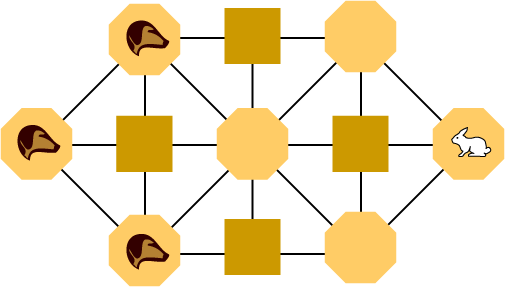
\includegraphics[width=.7\textwidth]{Hare_and_Hounds_board}
	\caption{The Hare and Hounds board.}
	\label{fig:board}
\end{figure}

We build a simulation where two players can play this game. The game has as
its inputs the positions of the animals, the output is where an animal moves
on a player's turn.

Since we are trying to teach a computer how to play a game the most reasonable
method to use is reinforcement learning. Because the game has a very small
state space it is not useful to train a supervised method because you would
need to calculate the optimal play for most of the states as training data.
If you have calculated this then you might as well implement a look up table
since the problem space is so small. Because we don't know what the optimal
move in each state is for either player we will use reinforcement learning
to discover these.

\section{Methods}
We implement two reinforcement learning players, one to play as the hounds
and one to play as the hare. We will use policy iteration to train both of the
implementations.

\section{Setup of experiments}
We will test the two implementations against opponents that make random moves.
We will also test the implementations against each other to see if the hounds
win in the plurality of cases since the game is biased towards the hounds. We
can also compare the found policies with the optimal policy.

\section{Programming language}
We are going to implement this project using Python 3.

\section{Planning}
\begin{center}
	\begin{tabular}{l|l}
		Date       & Objective                           \\ \hline
		2015-11-27 & Simulation working                  \\
		2015-12-04 &  \\
		2015-12-11 &  \\
		2015-12-16 & Writing reinforcement learning done \\
		2015-01-04 & Training done                       \\
		2016-01-08 & Experiment done                     \\
		2016-01-15 & Finish report
	\end{tabular}
\end{center}

\end{document}
